\chapter{Tests}
\label{chap:Tests}
Aus zeitlichen Gründen musste die Testphase gekürzt werden. Es konnten somit keine Testversuche auf dem Packpot durchgeführt werden. Nachfolgend wurden Funktionstests durchgeführt. Sie geben Einblick auf bestehende Mängel. 

\section{Testspezifikationen}
\label{sec:Testprotokolle}
Nachfolgende Tabelle, \ref{fig:funktest} gibt einen Überblick, welche Teilfunktion getestet werden. Dabei wird kurz ein Beschrieb dazu geliefert und welche Parameter bzw. Spezifikationen ausgewertet wurden. 

\begin{table}[H]
	\centering
	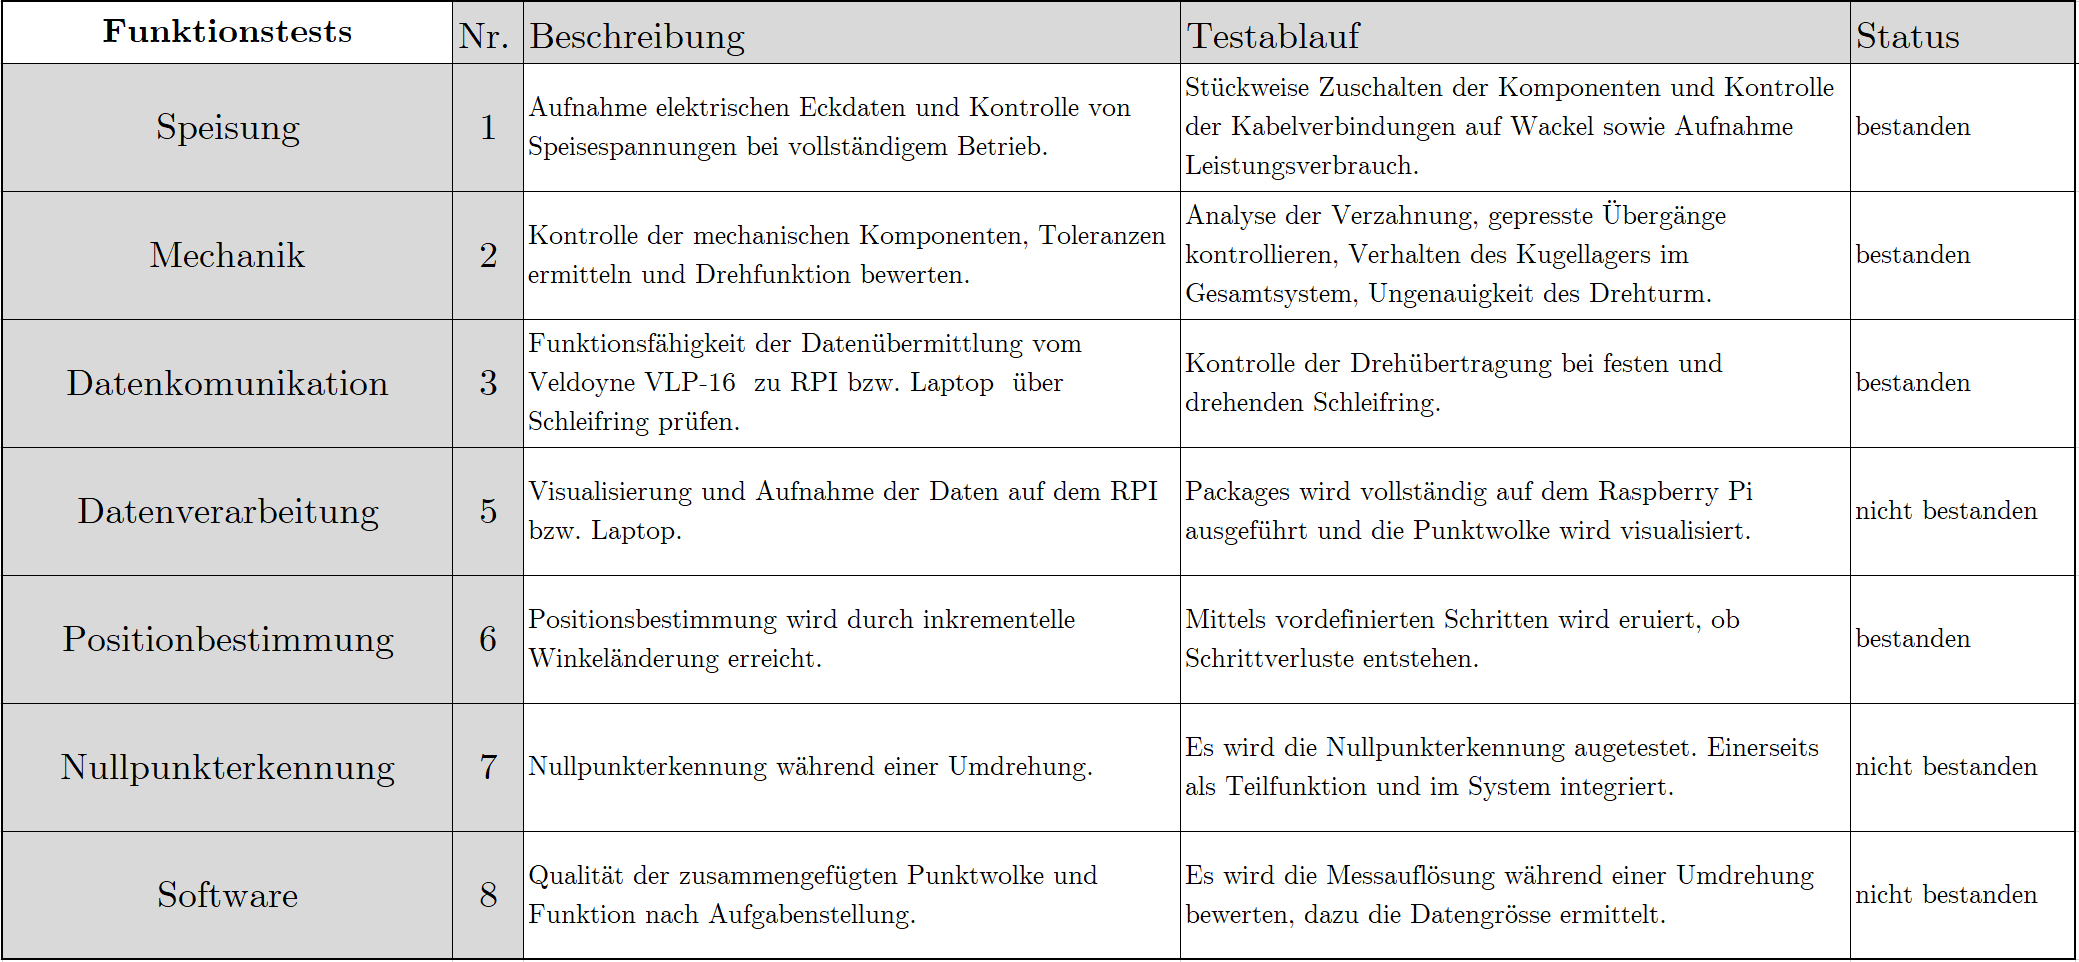
\includegraphics[,width=1\textwidth]{resources/Testtabelle.PNG}
	\caption[Funktionstest im Überblick]{Funktionstests im Überblick}
	\label{fig:funktest}
\end{table} 

\section {Testergebnisse}
\label{sec:Testergebnisse}
Die Testergebnisse zu den jeweiligen Funktionstests sind nachfolgend kurz beschrieben. Die Datensätze zu den entsprechenden Resultaten sind im Anhang in einem Excel-File einsehbar.

\subsection {T1: Speisung}
\label{subsec:Speisung}
Mittels einem Rohde \& Schwarz NGSM32 Netzteil wurde eine Speisung von 12.00 Volt zugeführt. Alle Komponenten konnten problemlos zugeschaltet werden. Wackelkontakte wurden keine festgestellt. Die Leistungsaufnahme des gesamten Prototyps variiert zwischen 12-15 Watt. Da keine Mängel festgestellt wurden, gilt dieser Funktionstest als erfüllt.
\subsection {T2: Mechanik}
\label{subsec:Mechanik}
Die Mechanik wurde auf Mängel geprüft. Die zwei Zahnräder verlaufen sehr exakt ineinander und verkanten sich nicht. Die gepressten Teile sitzen fest und verursachen keine Toleranzen. Einzig der Kugellageradapter ist nicht optimal gepresst. Dies verursacht, dass der drehende Hohlzylinder den Abstand zum QRE 1113 um einen Millimeter während der Drehung variiert. Da die Mechanik ansonsten einwandfrei funktioniert gilt dieser Funktionstest als bestanden.

\subsection {T3: Datenkommunikation}
\label{subsec:Datenkimmuikation}
Die Datenkommunikation ist in allen Fällen gewährleistet. Es kann zwischen dem Velodyne VLP-16, dem Raspberry Pi 3 und dem Laptop problemlos kommuniziert werden. Es wurden mehrere Datensätze auf vollständige Messages geprüft. Dabei konnten keine fehlenden Messages festgestellt werden. Die erstellten Datensätze wurden mit unrotierendem Turm, sowie mit den Drehgeschwindigkeiten von 5$^\circ$/s, 20$^\circ$/s und 120$^\circ$/s fehlerlos übermittelt.  

\subsection {T4: Datenverarbeitung}
\label{subsec:Datenverarbeitung}
Die Datenverarbeitung des Datenstreams wurde auf dem Raspberry Pi 3, wie auch auf dem Laptop geprüft. Beim Raspberry Pi 3 besteht das Problem, dass die Visualisierung mit Rviz mangelhaft funktioniert. Aufgrund der Datenrate von 8 Mbit/s steigt die Grösse der Punktwolke schnell an. Das Raspberry Pi stösst für die Visualisierung dieser Punktwolke an die Leistungsgrenzen. Auf dem Laptop werden die Punktwolke in Echtzeit visualisiert, da dieser bedeutend höhere Rechenleistungen bietet. 

\subsection {T5: Positionsbestimmung}
\label{subsec:Positionsbestimmung}
Die Positionsbestimmung wurde getestet, indem feste Schritte angefahren wurden. Mit der Umrechnung der Schrittzahl pro Umdrehung, lässt sich die Endpostion bestimmen. Dabei wird die Istposition mit der Sollposition verglichen. Aus der Differenz werden Schrittverluste ermittelt. Aus den Datensätzen stimmen die Sollwinkel mit den Istwinkel überein. Es wurden bei verschiedenen Drehgeschwindigkeiten 5$^\circ$/s, 20$^\circ$/s und 120$^\circ$/s) verschiedene Sollwinkel vorgegeben.

\subsection {T6: Nullpunkterkennung}
\label{subsec:testSNullpunkterkennung}
Der Nullpunkt wurde bei den Umdrehungsgeschwindigkeiten von 5$^\circ$/s, 20$^\circ$/s und 120$^\circ$/s nicht vollständig erkannt. Dabei wurden aus den erstellten Datensätzen festgestellt, dass bei 120$^\circ$/s die Nullpunkterkennung nur noch bei 13 von 24 Detektionen gelingt. Bei den anderen zwei Geschwindigkeiten sind lediglich eine bzw. zwei Erkennung fehlgeschlagen (23 von 24). Der Sensor wurde dazu mit einem KO verbunden, damit die Spannnungswerte getriggert werden konnten. Da die Nullposition nicht ständig gewährleistet ist, gilt dieser Test als gescheitert.

\subsection {T7: Software}
\label{subsec:testSoftware}
Die erstellte Software ermöglicht die Visualisierung einer zusammengefügten Punktwolke. Es können Punktwolken mit der maximalen Auflösung 0.3$^\circ$ beinahe kugelförmig aufgenommen werden. Lediglich ein Kegel von 90$^\circ$ nach unten wird von der Halterung verdeckt. Dies ist beabsichtigt, damit der Prototyp selbst nicht als Punktwolke visualisiert wird. Die Software ermöglicht jedoch nur die Visualisierung einer einzigen Umdrehung. Nach dem Löschen der Punktwolke, welche je nach Auflösung mehrere Gigabyte gross ist, kann die Software keine neuen Punkte speichern. Dieses Fehlverhalten ist Grund, dass der Test als nicht bestanden deklariert ist.

\section{Zwischenfazit}
\label{sec:Fazit}
Die Tests geben Überblick, welche Funktionsbereiche überarbeitet werden müssen, bzw. bei welchen noch nicht zufriedenstellende Ergebnisse geliefert werden.
Die Konstruktion bietet gute Ansätze, da die Mechanik, Datenkommunikation und Positionsbestimmung gewährleistet sind. Dabei ist die Leistungsaufnahme von maximal 15 Watt gering. Sie ermöglicht auch den Einsatz auf mobilen batteriebetriebenen Gefährten. Die Testergebnisse zeigen auf, dass für die Ansteuerung der Aktoren und Sensoren ein Raspberry Pi gute Dienste leistet. Für die Datenverarbeitung reicht das Raspberry Pi 3 nicht aus. Dafür wird eine leistungsfähigere Rechenmaschine benötigt. Die Nullpunkterkennung besitzt Mängel und ist nicht optimal gelöst. Auch die Software besitzt noch nicht die Qualität, um die Aufgabenstellung zu erfüllen.    